\section{Định nghĩa}
Internet là một mạng lưới phủ trên toàn thế giới, kết nối dữ liệu giữa các máy tính và các thiết bị liên quan. Internet là một “Chuyển mạch gói” (Packet Switched ) dữ liệu mạng, nghĩa là tin nhắn được gửi qua nó được chia thành các gói, các khối dữ liệu nhỏ, chúng được gửi qua mạng và ghép lại hoàn chỉnh ở đầu kia. Định dạng của các gói theo một tiêu chuẩn được gọi là Giao thức Internet (Internet Protocol-IP) và bao gồm một địa chỉ IP trong mỗi gói chỉ định đến đích của gói, nhờ đó mà nó có thể định tuyến chính xác vị trí trên mạng.\par
Thay thế cho mạng “Chuyển mạch gói”  là mạng “Chuyển mạch kênh” (Circuit Switched), ví dụ cơ bản là hệ thống điện thoại. Trong mạng chuyển mạch kênh, các mạch kết nối khi cần, chẳng hạn như khi một cuộc gọi được thực hiện, mạng sẽ phân bổ một mạch cho kết nối này, và chỉ dành riêng cho kết nối đến khi cuộc gọi kết thúc. Điều này hoạt động tốt trong hệ thống gọi thoại, với các cuộc gọi có điểm bắt đầu và kết thúc rõ ràng, tuy nhiên lại kém trong mạng dữ liệu, nơi mà việc truyền dữ liệu thường xuyên xảy ra những sự ngắt quãng, gián đoạn đột ngột. Sử dụng mô hình mạng chuyển mạch gói cho phép máy tính truyền và nhận những dữ liệu không liên tục hoặc ở các tốc độ truyền khác nhau mà không làm tăng dung lượng trên mạng. Bằng cách tách các gói nhỏ hợp lý, mạng cho phép một lượng nhất định các trường hợp lỗi. Không có gì lạ khi các gói biến mất trên Internet và không bao giờ đến đích, chỉ đôi khi là do lỗi phần cứng hay phần mềm, nhưng đa phần là do các gói bị xóa có chủ ý nhàm giảm tắc nghẽn trong những phần đang hoạt động bận rộn của mạng. Khi đó những tin nhắn chia thành nhiều gói sẽ bị mất một vài gói, và chỉ cần gửi lại những gói đã mất để hoàn thành tin nhắn thay vì gửi lại toàn bộ tin nhắn. Có một phần mềm được gọi là Transport Control Protocol (TCP) (Giao thức điều khiển và vận chuyển) chạy trên IP, nó tự động thực hiển kiểm tra và truyền nếu xảy ra lỗi mà không cần đến sự can thiệp từ người dùng máy tính hay một phần mềm nào khác.\par
Đại diện cơ bản nhất cho mạng Internet là các đỉnh của mạng đại diện cho các máy tính và thiết bị liên quan, còn các cạnh thì đại diện cho kết nối giữ chúng. Trên thực tế các máy tính thông thường chỉ chiếm các đỉnh bên ngoài mạng, các dữ liệu truyền đến và đi, chúng không đóng vai trò trung gian cho luồng dữ liệu giữa các mạng khác (Các máy tính thường chỉ kết nối duy nhất với mạng nên không nằm trên đường giữa bất kì máy tính nào khác). Các nút bên trong mạng Internet chủ yếu là các bộ đinh tuyến, máy tính chuyên dụng, nằm tại điểm nối giữa các dòng dữ liệu, chuyển tiếp gói dữ liệu theo hướng về đích dự định của chúng.\par

\section{Cấu trúc Internet dưới dạng sơ đồ}
Hình dạng tổng thể của Internet được hiển thị ở dạng sơ đồ trong hình \ref{fig:h21}. Mạng bao gồm ba cấp vòng tròn. Vòng tròn thứ nhất là cốt lõi của mạng, là xương sống (Backbone) của mạng, các đường trục cung cấp đường truyền dữ liệu băng thông đường dài toàn cầu, cùng với những bộ định tuyến hiệu suất cao, chúng được liên kết với nhau bởi trung tâm chuyển mạch. Backbone được vận hành bởi các nhà cung cấp (NBPs) (network backbone providers), chủ yếu là chính phủ các quốc gia và công ty truyền thông. \par
Vòng tròn thứ hai của mô hình Internet bao gồm các nhà cung cấp dịch vụ Internet hoặc ISPs, các công ty thương mại, chính phủ, trường đại học và những người có hợp đồng với NBPs để kết nối với xương sống và sau đó bán lại hoặc cung cấp kết nối đó cho người dùng, người tạo thành vòng tròn thứ ba, các doanh nghiệp, văn phòng chính phủ, học giả, người trong nhà, v.v. Trên thực tế, như hình \ref{fig:h21} cho thấy, các ISPs được chia nhỏ thành các ISPs khu vực và ISPs địa phương hoặc ISPs tiêu dùng, trước đây các tổ chức lớn có nhiều khách hàng là ISPs địa phương, những người lần lượt bán kết nối mạng cho người dùng. Tuy nhiên, sự khác biệt này có phần mờ nhạt, bởi vì các ISPs tiêu dùng lớn, như America Online hoặc British Telecom, thường hoạt động như các ISP khu vực của riêng họ (và một số cũng có thể là nhà cung cấp xương sống).
\begin{figure}[ht]
\centering
	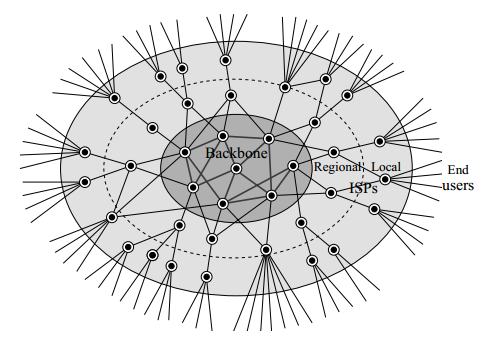
\includegraphics[width=0.5\textwidth]{res/h21.png}
	\caption{sơ đồ cấu trúc Internet: “Backbone”: xương sống của dải băng thông. ISPs: kết nối với “Backbone” và bị chia khoảng bởi Regional (Khu vực lớn) và Local (Địa phương nhỏ). End users: người dùng cá nhân, gia đình, công ty kết nối với ISPs.}
	\label{fig:h21}
\end{figure}

Cấu trúc mạng của Internet không bị quy định bởi bất kỳ cơ quan trung ương nào. Các giao thức và hướng dẫn được phát triển bởi một tổ chức tình nguyện không chính thức có tên là Internet Engineering Task Force, họ không phải nộp đơn cho bất kỳ cơ quan Internet trung ương nào để xin phép xây dựng một mạng mới trên Internet hoặc đưa ra khỏi dịch vụ.\par
Một trong những tính năng đáng chú ý của Internet là sơ đồ được sử dụng để định tuyến các gói từ đích này đến đích khác được đưa ra bằng cách trao đổi tự động giữa các bộ định tuyến Internet bằng cách sử dụng một hệ thống gọi là Giao thức cổng biên (Border Gateway Protocol- BGP). BGP được thiết kế theo cách nếu các đỉnh hoặc cạnh mới được thêm vào mạng, các đỉnh cũ biến mất, các điểm hiện tại bị hỏng vĩnh viễn hoặc tạm thời, các bộ định tuyến sẽ lưu ý và điều chỉnh hệ thống định tuyến của chúng một cách thích hợp. Một số hoạt động cần con người giám sát để đảm bảo sự trơn tru, nhưng không cần có “chính quyền Internet” nào để điều khiển mọi thứ từ trên cao, hệ thống tự tổ chức bằng cách kết hợp hoạt động của hệ thống máy tính địa phương cơ bản tự động.\par
Mặc dù đây là một tính năng tuyệt vời của hệ thống với sự mạnh mẽ và linh hoạt, nhưng nó là một vấn đề đối với những người muốn nghiên cứu cấu trúc của Internet, bởi vì không có đăng ký trung tâm nào mà người ta có thể xác định cấu trúc đó. Không có ai có nhiệm vụ duy trì một bản đồ chính thức của mạng. Thay vào đó, cấu trúc mạng phải được xác định bằng các phép đo thử nghiệm. Có hai phương pháp chính để làm điều này. Cách một là “traceroute”, cách hai là sử dụng BGP.\par
